\section{Sistema D – Sistema de Segurança}

É fundamental para o sistema que a cada movimento detetado seja `disparado' um alarme sonoro em conjunto com um LED intermitente. Mais ainda, deve ser possível terminar o alarme com o pressionar de um botão.

Como tal, considerando a importância de cada ação, foi decidida a implementação de ambas em torno do conceito de interrupção do sistema.

\begin{figure}[H]
    \centering
    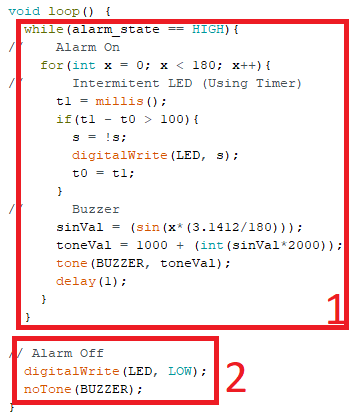
\includegraphics{images/codigo/sisD_loop.png}
    \caption{Função loop()}
    \label{fig:my_label}
\end{figure}

Podemos verificar que o Programa apenas executa:
\begin{enumerate}
    \item A funcionalidade de alarme, quando o alarme estiver acionado
    \item Suspensão de alarme
\end{enumerate}

As seguintes funções são chamadas por interrupts acionados pelo Sensor PIR e um botão, respetivamente.

\begin{figure}[H]
    \centering
    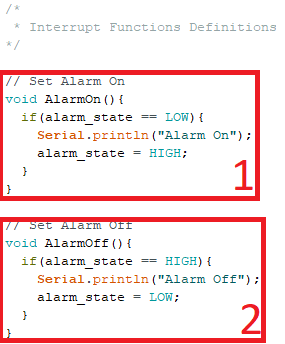
\includegraphics{images/codigo/sisD_interrupts.png}
    \caption{Funções de Chamadas de Interrupt}
    \label{fig:my_label}
\end{figure}


\begin{enumerate}
    \item \textbf{AlarmOn()} -- Chamada por movimento detetado pelo Sensor.
    \item \textbf{AlarmOff()} -- Chamada por pressão de botão.
\end{enumerate}